\documentclass{amsart}
\usepackage{graphicx}
\title{Keyboard Layout Analyzer Manual}
\begin{document}
\maketitle
\begin{abstract}
KLA is a Qt software for analyzing keyboard layouts.
\end{abstract}
\section{Copyright}
Copyright (C) 2013  Omid Nikta, EMail: \verb+omidnikta@gmail.com+

This program is free software: you can redistribute it and/or modify
it under the terms of the GNU General Public License as published by
the Free Software Foundation, either version 3 of the License, or
(at your option) any later version.

This program is distributed in the hope that it will be useful,
but WITHOUT ANY WARRANTY; without even the implied warranty of
MERCHANTABILITY or FITNESS FOR A PARTICULAR PURPOSE.  See the
GNU General Public License for more details.

You should have received a copy of the GNU General Public License
along with this program.  If not, see \verb+http://www.gnu.org/licenses/+.
\section{How to use}
A keyboard layout file is a plain text file. The first line contains the name
and the second line contain all the characters in the layout (better to be ordered). 
The third line is important. You should put all the characters in the layout, separated by space and 
then you should define the position of the characters after the line that looks like this:
\begin{verbatim}
Row 	Finger      Move        Shift
\end{verbatim}
For example the character `T' on the QWERTY keyboard is shown this way
\begin{verbatim}
1     3     1      0
\end{verbatim}
It means that `T' is on the first row, is hitted by finger 3, the figer must move a block to right, and needs shift.
The rows enumerated from -1 to 2. On the QWERTY layout,  rows that contain `z', `a', `q', 1' are -1, 0, 1, 2, respectively. See Figure \ref{rows.jpg} for more info.
\begin{figure}[!ht]
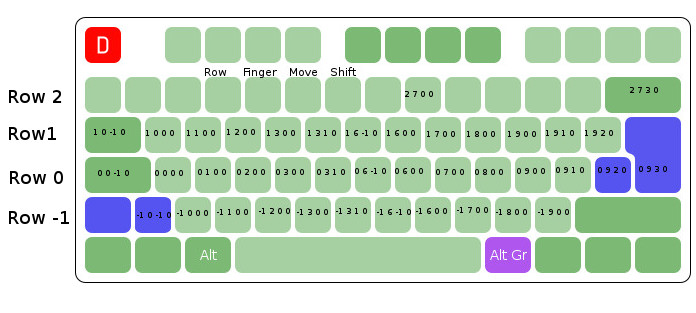
\includegraphics[height=6cm]{rows.jpg}
\caption{Rows explanation}\label{rows}
\end{figure}

Figure \ref{layoutfile} is an example of the QWERTY keyboard on a ANSI standard keyboard:
\begin{figure}[!ht]
\begin{verbatim}
US(QWERTY)
a b c d e f g h i j k l m n o p q r s t u v w x y z , . ; : ?
q w e r t y u i o p a s d f g h j k l ; z x c v b n m , . / Q W E R T Y ... V B N M < > ?
Row           Finger            Move             Shift
1                0                0                0
1                1                0                0
1                2                0                0 
1                3                0                0
1                3                1                0
1                6               -1                0
1                6                0                0
.
.
.
-1                7               0                1
-1                8               0                1
-1                9               0                1
0                 5               0                0
0                 9               3                0

\end{verbatim}
\caption{A sample layout file}\label{layoutfile}
\end{figure}
\begin{figure}[!ht]
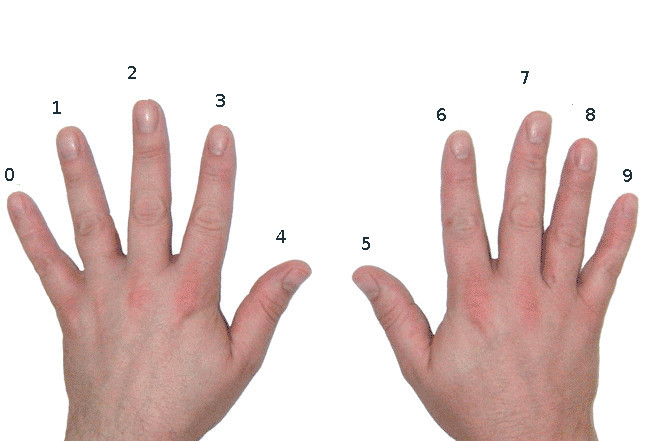
\includegraphics[height=5cm]{fingers.jpg}
\caption{Fingers Numbers}\label{fingers}
\end{figure}
The information after (Row 	Finger 	Move Shift) row is the same order that you enter
the characters. For example the first character is ` which its information comes first, 
i.e, \verb+2	   0    -1    0+ which means its on the row 2, is hitted by finger 0,
the corresponding finger needs to move one block horizontally to left (normally the finger 0, 
left pinky, hit key 1, so it must move a block left to reach `), and the last 0 means that it doesn't need shift (put 1 if it needs shift).

Another examples: w " b B

\begin{verbatim}
1    1   0   0
0    9   1   1
-1   3   1   0
-1   3   1   1
\end{verbatim}

{\bfseries Important:} The last two line of the file is for space and return. They are of the following
form on an ANSI keyboard

\begin{verbatim}
0   5   0   0
0   9   2   0
\end{verbatim}
and of the following form on an ISO keyboard

\begin{verbatim}
0   5   0   0
0   9   3   0
\end{verbatim}

Good news is that you normally don't need to write a layout file from scrach. I have created well-known layouts,
QWERTY, COLEMAK, WORKMAN and DVORAK. You just need to choose any of these file and just replace the 
set of characters (third line) with your choice. Yes, It is that simple.

\end{document}